% Options for packages loaded elsewhere
% Options for packages loaded elsewhere
\PassOptionsToPackage{unicode}{hyperref}
\PassOptionsToPackage{hyphens}{url}
\PassOptionsToPackage{dvipsnames,svgnames,x11names}{xcolor}
%
\documentclass[
  letterpaper,
  DIV=11,
  numbers=noendperiod]{scrartcl}
\usepackage{xcolor}
\usepackage{amsmath,amssymb}
\setcounter{secnumdepth}{5}
\usepackage{iftex}
\ifPDFTeX
  \usepackage[T1]{fontenc}
  \usepackage[utf8]{inputenc}
  \usepackage{textcomp} % provide euro and other symbols
\else % if luatex or xetex
  \usepackage{unicode-math} % this also loads fontspec
  \defaultfontfeatures{Scale=MatchLowercase}
  \defaultfontfeatures[\rmfamily]{Ligatures=TeX,Scale=1}
\fi
\usepackage{lmodern}
\ifPDFTeX\else
  % xetex/luatex font selection
\fi
% Use upquote if available, for straight quotes in verbatim environments
\IfFileExists{upquote.sty}{\usepackage{upquote}}{}
\IfFileExists{microtype.sty}{% use microtype if available
  \usepackage[]{microtype}
  \UseMicrotypeSet[protrusion]{basicmath} % disable protrusion for tt fonts
}{}
\makeatletter
\@ifundefined{KOMAClassName}{% if non-KOMA class
  \IfFileExists{parskip.sty}{%
    \usepackage{parskip}
  }{% else
    \setlength{\parindent}{0pt}
    \setlength{\parskip}{6pt plus 2pt minus 1pt}}
}{% if KOMA class
  \KOMAoptions{parskip=half}}
\makeatother
% Make \paragraph and \subparagraph free-standing
\makeatletter
\ifx\paragraph\undefined\else
  \let\oldparagraph\paragraph
  \renewcommand{\paragraph}{
    \@ifstar
      \xxxParagraphStar
      \xxxParagraphNoStar
  }
  \newcommand{\xxxParagraphStar}[1]{\oldparagraph*{#1}\mbox{}}
  \newcommand{\xxxParagraphNoStar}[1]{\oldparagraph{#1}\mbox{}}
\fi
\ifx\subparagraph\undefined\else
  \let\oldsubparagraph\subparagraph
  \renewcommand{\subparagraph}{
    \@ifstar
      \xxxSubParagraphStar
      \xxxSubParagraphNoStar
  }
  \newcommand{\xxxSubParagraphStar}[1]{\oldsubparagraph*{#1}\mbox{}}
  \newcommand{\xxxSubParagraphNoStar}[1]{\oldsubparagraph{#1}\mbox{}}
\fi
\makeatother


\usepackage{longtable,booktabs,array}
\usepackage{calc} % for calculating minipage widths
% Correct order of tables after \paragraph or \subparagraph
\usepackage{etoolbox}
\makeatletter
\patchcmd\longtable{\par}{\if@noskipsec\mbox{}\fi\par}{}{}
\makeatother
% Allow footnotes in longtable head/foot
\IfFileExists{footnotehyper.sty}{\usepackage{footnotehyper}}{\usepackage{footnote}}
\makesavenoteenv{longtable}
\usepackage{graphicx}
\makeatletter
\newsavebox\pandoc@box
\newcommand*\pandocbounded[1]{% scales image to fit in text height/width
  \sbox\pandoc@box{#1}%
  \Gscale@div\@tempa{\textheight}{\dimexpr\ht\pandoc@box+\dp\pandoc@box\relax}%
  \Gscale@div\@tempb{\linewidth}{\wd\pandoc@box}%
  \ifdim\@tempb\p@<\@tempa\p@\let\@tempa\@tempb\fi% select the smaller of both
  \ifdim\@tempa\p@<\p@\scalebox{\@tempa}{\usebox\pandoc@box}%
  \else\usebox{\pandoc@box}%
  \fi%
}
% Set default figure placement to htbp
\def\fps@figure{htbp}
\makeatother


% definitions for citeproc citations
\NewDocumentCommand\citeproctext{}{}
\NewDocumentCommand\citeproc{mm}{%
  \begingroup\def\citeproctext{#2}\cite{#1}\endgroup}
\makeatletter
 % allow citations to break across lines
 \let\@cite@ofmt\@firstofone
 % avoid brackets around text for \cite:
 \def\@biblabel#1{}
 \def\@cite#1#2{{#1\if@tempswa , #2\fi}}
\makeatother
\newlength{\cslhangindent}
\setlength{\cslhangindent}{1.5em}
\newlength{\csllabelwidth}
\setlength{\csllabelwidth}{3em}
\newenvironment{CSLReferences}[2] % #1 hanging-indent, #2 entry-spacing
 {\begin{list}{}{%
  \setlength{\itemindent}{0pt}
  \setlength{\leftmargin}{0pt}
  \setlength{\parsep}{0pt}
  % turn on hanging indent if param 1 is 1
  \ifodd #1
   \setlength{\leftmargin}{\cslhangindent}
   \setlength{\itemindent}{-1\cslhangindent}
  \fi
  % set entry spacing
  \setlength{\itemsep}{#2\baselineskip}}}
 {\end{list}}
\usepackage{calc}
\newcommand{\CSLBlock}[1]{\hfill\break\parbox[t]{\linewidth}{\strut\ignorespaces#1\strut}}
\newcommand{\CSLLeftMargin}[1]{\parbox[t]{\csllabelwidth}{\strut#1\strut}}
\newcommand{\CSLRightInline}[1]{\parbox[t]{\linewidth - \csllabelwidth}{\strut#1\strut}}
\newcommand{\CSLIndent}[1]{\hspace{\cslhangindent}#1}



\setlength{\emergencystretch}{3em} % prevent overfull lines

\providecommand{\tightlist}{%
  \setlength{\itemsep}{0pt}\setlength{\parskip}{0pt}}



 


\KOMAoption{captions}{tableheading}
\usepackage{blkarray}

\newcommand{\bzero}{{\mathbf 0}}
\newcommand{\bone}{{\mathbf 1}}
\newcommand{\ba}{{\mathbf a}}
\newcommand{\bb}{{\mathbf b}}
\newcommand{\bc}{{\mathbf c}}
\newcommand{\bd}{{\mathbf d}}
\newcommand{\be}{{\mathbf e}}
\newcommand{\bff}{{\mathbf f}}
\newcommand{\bg}{{\mathbf g}}
\newcommand{\bh}{{\mathbf h}}
\newcommand{\bi}{{\mathbf i}}
\newcommand{\bj}{{\mathbf j}}
\newcommand{\bk}{{\mathbf k}}
\newcommand{\bl}{{\mathbf l}}
\newcommand{\bmm}{{\mathbf m}}
\newcommand{\bn}{{\mathbf n}}
\newcommand{\bo}{{\mathbf o}}
\newcommand{\bp}{{\mathbf p}}
\newcommand{\bq}{{\mathbf q}}
\newcommand{\br}{{\mathbf r}}
\newcommand{\bs}{{\mathbf s}}
\newcommand{\bt}{{\mathbf t}}
\newcommand{\bu}{{\mathbf u}}
\newcommand{\bv}{{\mathbf v}}
\newcommand{\bw}{{\mathbf w}}
\newcommand{\bx}{{\mathbf x}}
\newcommand{\by}{{\mathbf y}}
\newcommand{\bz}{{\mathbf z}}
\newcommand{\bA}{{\mathbf A}}
\newcommand{\bB}{{\mathbf B}}
\newcommand{\bC}{{\mathbf C}}
\newcommand{\bD}{{\mathbf D}}
\newcommand{\bE}{{\mathbf E}}
\newcommand{\bF}{{\mathbf F}}
\newcommand{\bG}{{\mathbf G}}
\newcommand{\bH}{{\mathbf H}}
\newcommand{\bI}{{\mathbf I}}
\newcommand{\bJ}{{\mathbf J}}
\newcommand{\bK}{{\mathbf K}}
\newcommand{\bL}{{\mathbf L}}
\newcommand{\bM}{{\mathbf M}}
\newcommand{\bN}{{\mathbf N}}
\newcommand{\bO}{{\mathbf O}}
\newcommand{\bP}{{\mathbf P}}
\newcommand{\bQ}{{\mathbf Q}}
\newcommand{\bR}{{\mathbf R}}
\newcommand{\bS}{{\mathbf S}}
\newcommand{\bT}{{\mathbf T}}
\newcommand{\bU}{{\mathbf U}}
\newcommand{\bV}{{\mathbf V}}
\newcommand{\bW}{{\mathbf W}}
\newcommand{\bX}{{\mathbf X}}
\newcommand{\bY}{{\mathbf Y}}
\newcommand{\bZ}{{\mathbf Z}}
\newcommand{\balpha}{{\boldsymbol\alpha}}
\newcommand{\bbeta}{{\boldsymbol\beta}}
\newcommand{\bgamma}{{\boldsymbol\gamma}}
\newcommand{\bdelta}{{\boldsymbol\delta}}
\newcommand{\bepsilon}{{\boldsymbol\epsilon}}
\newcommand{\bvarepsilon}{{\boldsymbol\varepsilon}}
\newcommand{\bzeta}{{\boldsymbol\zeta}}
\newcommand{\bfeta}{{\boldsymbol\eta}}
\newcommand{\boldeta}{{\boldsymbol\eta}}
\newcommand{\btheta}{{\boldsymbol\theta}}
\newcommand{\bvartheta}{{\boldsymbol\vartheta}}
\newcommand{\biota}{{\boldsymbol\iota}}
\newcommand{\bkappa}{{\boldsymbol\kappa}}
\newcommand{\blambda}{{\boldsymbol\lambda}}
\newcommand{\bmu}{{\boldsymbol\mu}}
\newcommand{\bnu}{{\boldsymbol\nu}}
\newcommand{\bxi}{{\boldsymbol\xi}}
\newcommand{\bpi}{{\boldsymbol\pi}}
\newcommand{\bvarpi}{{\boldsymbol\varpi}}
\newcommand{\brho}{{\boldsymbol\rho}}
\newcommand{\bvarrho}{{\boldsymbol\varrho}}
\newcommand{\bsigma}{{\boldsymbol\sigma}}
\newcommand{\bvarsigma}{{\boldsymbol\varsigma}}
\newcommand{\btau}{{\boldsymbol\tau}}
\newcommand{\bupsilon}{{\boldsymbol\upsilon}}
\newcommand{\bphi}{{\boldsymbol\phi}}
\newcommand{\bvarphi}{{\boldsymbol\varphi}}
\newcommand{\bchi}{{\boldsymbol\chi}}
\newcommand{\bpsi}{{\boldsymbol\psi}}
\newcommand{\bomega}{{\boldsymbol\omega}}
\newcommand{\bGamma}{{\boldsymbol\Gamma}}
\newcommand{\bDelta}{{\boldsymbol\Delta}}
\newcommand{\bTheta}{{\boldsymbol\Theta}}
\newcommand{\bLambda}{{\boldsymbol\Lambda}}
\newcommand{\bXi}{{\boldsymbol\Xi}}
\newcommand{\bPi}{{\boldsymbol\Pi}}
\newcommand{\bSigma}{{\boldsymbol\Sigma}}
\newcommand{\bUpsilon}{{\boldsymbol\Upsilon}}
\newcommand{\bPhi}{{\boldsymbol\Phi}}
\newcommand{\bPsi}{{\boldsymbol\Psi}}
\newcommand{\bOmega}{{\boldsymbol\Omega}}
\DeclareMathOperator{\diag}{diag}
\DeclareMathOperator{\Prob}{P}
\DeclareMathOperator{\E}{E}
\DeclareMathOperator{\Var}{Var}
\DeclareMathOperator{\Cov}{Cov}
\DeclareMathOperator{\Corr}{Corr}
\DeclareMathOperator{\sd}{sd}
\DeclareMathOperator{\se}{se}
\DeclareMathOperator{\N}{N}
\DeclareMathOperator{\Bin}{Bin}
\DeclareMathOperator{\Bern}{Bern}
\DeclareMathOperator{\Dir}{Dir}
\DeclareMathOperator{\Wis}{Wis}
\DeclareMathOperator{\logit}{logit}
\DeclareMathOperator{\expit}{expit}
\DeclareMathOperator{\Mult}{Mult}
\DeclareMathOperator{\Cat}{Cat}
\DeclareMathOperator{\Pois}{Poi}
\DeclareMathOperator{\Geom}{Geom}
\DeclareMathOperator{\NBin}{NBin}
\DeclareMathOperator{\Exp}{Exp}
\DeclareMathOperator{\Betadist}{Beta}
\DeclareMathOperator{\Hypergeom}{Hypergeom}
\DeclareMathOperator{\Cauchy}{Cauchy}
\DeclareMathOperator{\hCauchy}{half-Cauchy}
\DeclareMathOperator{\LKJ}{LKJ}
\DeclareMathOperator{\Unif}{Unif}
\DeclareMathOperator{\KL}{KL}
\DeclareMathOperator{\ind}{\mathds{1}}
\newcommand{\iid}{\,\overset{\text{iid}}{\sim}\,}
\DeclareMathOperator*{\plim}{plim}
\DeclareMathOperator{\Lik}{L}
\DeclareMathOperator{\argmax}{argmax}
\DeclareMathOperator{\vecc}{vec}
\DeclareMathOperator{\dd}{d}
\newcommand{\dint}{\dd\hspace{0.5pt}\!}

\newcommand{\bbR}{\mathbb{R}}
\newcommand{\bbN}{\mathbb{N}}
\newcommand{\bbZ}{\mathbb{Z}}
\newcommand{\bbC}{\mathbb{C}}
\newcommand{\bbS}{\mathbb{S}}
\newcommand{\bbH}{\mathbb{H}}
\newcommand{\bbP}{\mathbb{P}}

\newcommand{\cA}{{\mathcal A}}
\newcommand{\cB}{{\mathcal B}}
\newcommand{\cC}{{\mathcal C}}
\newcommand{\cD}{{\mathcal D}}
\newcommand{\cE}{{\mathcal E}}
\newcommand{\cF}{{\mathcal F}}
\newcommand{\cG}{{\mathcal G}}
\newcommand{\cH}{{\mathcal H}}
\newcommand{\cI}{{\mathcal I}}
\newcommand{\cJ}{{\mathcal J}}
\newcommand{\cK}{{\mathcal K}}
\newcommand{\cL}{{\mathcal L}}
\newcommand{\cM}{{\mathcal M}}
\newcommand{\cN}{{\mathcal N}}
\newcommand{\cO}{{\mathcal O}}
\newcommand{\cP}{{\mathcal P}}
\newcommand{\cQ}{{\mathcal Q}}
\newcommand{\cR}{{\mathcal R}}
\newcommand{\cS}{{\mathcal S}}
\newcommand{\cT}{{\mathcal T}}
\newcommand{\cU}{{\mathcal U}}
\newcommand{\cV}{{\mathcal V}}
\newcommand{\cW}{{\mathcal W}}
\newcommand{\cX}{{\mathcal X}}
\newcommand{\cY}{{\mathcal Y}}
\newcommand{\cZ}{{\mathcal Z}}

\newcommand{\myoverbrace}[3][gray]{{\color{#1}\overbrace{\color{black}#2}^{#3}}}
\newcommand{\myunderbrace}[3][gray]{{\color{#1}\underbrace{\color{black}#2}_{#3}}}

\makeatletter
\@ifpackageloaded{caption}{}{\usepackage{caption}}
\AtBeginDocument{%
\ifdefined\contentsname
  \renewcommand*\contentsname{Table of contents}
\else
  \newcommand\contentsname{Table of contents}
\fi
\ifdefined\listfigurename
  \renewcommand*\listfigurename{List of Figures}
\else
  \newcommand\listfigurename{List of Figures}
\fi
\ifdefined\listtablename
  \renewcommand*\listtablename{List of Tables}
\else
  \newcommand\listtablename{List of Tables}
\fi
\ifdefined\figurename
  \renewcommand*\figurename{Figure}
\else
  \newcommand\figurename{Figure}
\fi
\ifdefined\tablename
  \renewcommand*\tablename{Table}
\else
  \newcommand\tablename{Table}
\fi
}
\@ifpackageloaded{float}{}{\usepackage{float}}
\floatstyle{ruled}
\@ifundefined{c@chapter}{\newfloat{codelisting}{h}{lop}}{\newfloat{codelisting}{h}{lop}[chapter]}
\floatname{codelisting}{Listing}
\newcommand*\listoflistings{\listof{codelisting}{List of Listings}}
\usepackage{amsthm}
\theoremstyle{plain}
\newtheorem{theorem}{Theorem}[section]
\theoremstyle{remark}
\AtBeginDocument{\renewcommand*{\proofname}{Proof}}
\newtheorem*{remark}{Remark}
\newtheorem*{solution}{Solution}
\newtheorem{refremark}{Remark}[section]
\newtheorem{refsolution}{Solution}[section]
\makeatother
\makeatletter
\makeatother
\makeatletter
\@ifpackageloaded{caption}{}{\usepackage{caption}}
\@ifpackageloaded{subcaption}{}{\usepackage{subcaption}}
\makeatother
\usepackage{bookmark}
\IfFileExists{xurl.sty}{\usepackage{xurl}}{} % add URL line breaks if available
\urlstyle{same}
\hypersetup{
  pdftitle={A title},
  pdfkeywords={Keyword, Keyword, Keyword, Keyword, Keyword},
  colorlinks=true,
  linkcolor={blue},
  filecolor={Maroon},
  citecolor={Blue},
  urlcolor={Blue},
  pdfcreator={LaTeX via pandoc}}


\title{A title}
\author{Haziq Jamil \and Another Coauthor}
\date{}
\begin{document}
\maketitle
\begin{abstract}
A nice abstract goes here.
\end{abstract}


\section{Introduction}\label{introduction}

The structural equation models are
\begin{equation}\phantomsection\label{eq-sem}{
\begin{aligned}
  \by &= \bnu + \bLambda \bfeta + \bepsilon \\
  \bfeta &= \balpha + \bB \bfeta  + \bzeta \\
  \bepsilon &\sim \N(\bzero, \bTheta_{\bepsilon}) \\
  \bzeta &\sim \N(\bzero, \bPsi) \\
\end{aligned}
}\end{equation}

where \(\bLambda\) is the factor loading matrix, \(\bfeta\) is the
latent variable vector, \(\bepsilon\) is the measurement error vector,
\(\bnu\) is the intercept vector, \(\balpha\) is the intercept vector
for the latent variables, \(\bB\) is the regression coefficient matrix
for the latent variables, and \(\bTheta_{\bepsilon}\) and \(\bPsi\) are
the covariance matrices of the measurement errors and latent variables,
respectively. The model defined by Equation~\ref{eq-sem} is very nice.

\section{Methods}\label{methods}

Lorem ipsum dolor sit amet, consectetur adipiscing elit. Duis sagittis
posuere ligula sit amet lacinia. Duis dignissim pellentesque magna,
rhoncus congue sapien finibus mollis. Ut eu sem laoreet, vehicula ipsum
in, convallis erat. Vestibulum magna sem, blandit pulvinar augue sit
amet, auctor malesuada sapien. Nullam faucibus leo eget eros hendrerit,
non laoreet ipsum lacinia. Curabitur cursus diam elit, non tempus ante
volutpat a. Quisque hendrerit blandit purus non fringilla. Integer sit
amet elit viverra ante dapibus semper. Vestibulum viverra rutrum enim,
at luctus enim posuere eu. Orci varius natoque penatibus et magnis dis
parturient montes, nascetur ridiculus mus.

Nunc ac dignissim magna. Vestibulum vitae egestas elit. Proin feugiat
leo quis ante condimentum, eu ornare mauris feugiat. Pellentesque
habitant morbi tristique senectus et netus et malesuada fames ac turpis
egestas. Mauris cursus laoreet ex, dignissim bibendum est posuere
iaculis. Suspendisse et maximus elit. In fringilla gravida ornare.
Aenean id lectus pulvinar, sagittis felis nec, rutrum risus. Nam vel
neque eu arcu blandit fringilla et in quam. Aliquam luctus est sit amet
vestibulum eleifend. Phasellus elementum sagittis molestie. Proin tempor
lorem arcu, at condimentum purus volutpat eu. Fusce et pellentesque
ligula. Pellentesque id tellus at erat luctus fringilla. Suspendisse
potenti.

\begin{figure}

\centering{

\pandocbounded{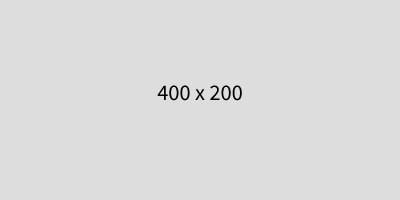
\includegraphics[keepaspectratio]{manuscript_files/mediabag/Beo6Fv01AACgREABKBAS.png}}

}

\caption{\label{fig-placeholder}Here's a caption.}

\end{figure}%

We need to update Figure~\ref{fig-placeholder} to a better one in the
future!

\section*{References}\label{references}
\addcontentsline{toc}{section}{References}

\phantomsection\label{refs}
\begin{CSLReferences}{1}{0}
\bibitem[\citeproctext]{ref-bartholomew2011latent}
Bartholomew, D. J., Knott, M., \& Moustaki, I. (2011). \emph{Latent
variable models and factor analysis: A unified approach} (3rd ed).
Wiley.

\bibitem[\citeproctext]{ref-bollen1989structural}
Bollen, K. A. (1989). \emph{Structural equations with latent variables}
(pp. xiv, 514). John Wiley \& Sons.
\url{https://doi.org/10.1002/9781118619179}

\bibitem[\citeproctext]{ref-joreskog2001factor}
Jöreskog, K. G., \& Moustaki, I. (2001). Factor {Analysis} of {Ordinal
Variables}: {A Comparison} of {Three Approaches}. \emph{Multivariate
Behavioral Research}, \emph{36}(3), 347--387.
\url{https://doi.org/10.1207/S15327906347-387}

\bibitem[\citeproctext]{ref-lee2007structural}
Lee, S.-Y. (2007). \emph{Structural equation modeling: A {Bayesian}
approach}. Wiley.

\bibitem[\citeproctext]{ref-rue2009approximate}
Rue, H., Martino, S., \& Chopin, N. (2009). Approximate {Bayesian
Inference} for {Latent Gaussian} models by using {Integrated Nested
Laplace Approximations}. \emph{Journal of the Royal Statistical Society
Series B: Statistical Methodology}, \emph{71}(2), 319--392.
\url{https://doi.org/10.1111/j.1467-9868.2008.00700.x}

\end{CSLReferences}

\section*{Appendix}\label{appendix}
\addcontentsline{toc}{section}{Appendix}

\section{Derivatives}\label{derivatives}

\[
\begin{aligned}
\frac{\partial \ell(\theta)}{\partial \theta} 
&= \frac{\partial}{\partial \theta} \left( \sum_{i=1}^{n} \log p(x_i | \theta) \right)\\
&= \sum_{i=1}^{n} \frac{\partial}{\partial \theta} \log p(x_i | \theta) \\
&= \sum_{i=1}^{n} \frac{1}{p(x_i | \theta)} \frac{\partial p(x_i | \theta)}{\partial \theta}
\end{aligned}
\]

\section{Additional proof}\label{additional-proof}

Please look at Theorem~\ref{thm-prime}.

\begin{theorem}[]\protect\hypertarget{thm-prime}{}\label{thm-prime}

There are an in finite number of primes.

\end{theorem}

\begin{proof}
Assume there are a finite number of primes, say
\(p_1, p_2, \ldots, p_n\). Consider the number
\(N = p_1 p_2 \cdots p_n + 1\). This number is not divisible by any of
the primes \(p_1, p_2, \ldots, p_n\) (since it leaves a remainder of 1
when divided by any of them). Therefore, \(N\) must either be prime
itself or have a prime factor that is not in our original list,
contradicting the assumption that we had listed all primes. Thus, there
are an infinite number of primes.
\end{proof}




\end{document}
